\chapter{\label{chap:szenarien}Szenarien im Ampelbereich}
Alle in Kapitel \ref{chap:state} angeführten Studien zu Ampelinformationssystemen und Konzepte zu Fahrraderweiterungen haben die Gemeinsamkeit des selbstkontrontollierten Fahrverhaltens der FahrerInnen. Ausgesprochen werden lediglich Empfehlungen, die möglichst intuitiv und schnell vermittelt werden. Grundlegend sollte die Anwendung in der Lage sein, die passende Empfehlung oder Handlungsaufforderung anzuzeigen, die sich aus folgenden Szenarien ergeben.
\begin{figure}[H]  
    \centering  
    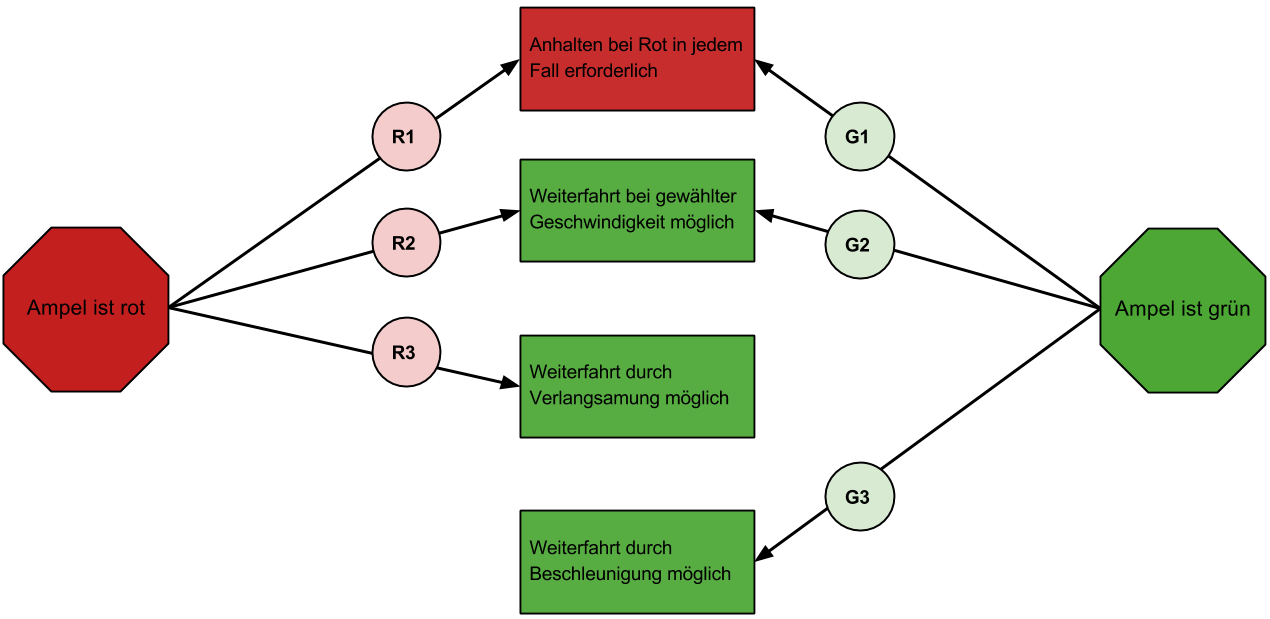
\includegraphics[width=1\textwidth]{Use-Cases} 
    \rule{35em}{0.5pt}
    \caption[Szenarien]{Szenarien im Ampelbereich}
    \label{fig:szenarien}
\end{figure}
\begin{description}[leftmargin=0.7cm,style=nextline]
% ROT
\item[Szenario R1:] 
Die Fahrradfahrerin oder der Fahrradfahrer nähert sich einer roten Ampel. Die Anwendung zeigt den Countdown der Restrotzeit an und empfieht langsamer zu fahren, um die Ampel ohne anzuhalten passieren zu können.  \\
\item[Szenario R2:] 
Die Fahrradfahrerin oder der Fahrradfahrer nähert sich einer roten Ampel. Die Anwendung zeigt an, es besteht kein Aktionsbedarf und eine Weiterfahrt bei gleichbleibender Geschwindigkeit ist gewährleistet. \\
\item[Szenario R3:] 
Die Fahrradfahrerin oder der Fahrradfahrer nähert sich einer roten Ampel. Die Anwendung meldet, das Anhalten bei roter Ampel ist in jedem Fall erforderlich.\\
% GRÜN 
\item[Szenario G1:] 
Die Fahrradfahrerin oder der Fahrradfahrer nähert sich einer grünen Ampel. Die Anwendung zeigt den Countdown der Restgrünzeit an und empfieht schneller zu fahren, um die Ampel ohne anzuhalten passieren zu können.\\
\item[Szenario G2:] 
Die Fahrradfahrerin oder der Fahrradfahrer nähert sich einer grünen Ampel. Die Anwendung zeigt an, es besteht kein Aktionsbedarf und eine Weiterfahrt bei gleichbleibender Geschwindigkeit ist gewährleistet.\\ 
\item[Szenario G3:] 
Die Fahrradfahrerin oder der Fahrradfahrer nähert sich einer grünen Ampel. Die Anwendung meldet, das Anhalten bei roter Ampel ist in jedem Fall erforderlich, da eine unrealistisch hohe Geschwindigkeit zum Erreichen der grünen Ampel erforderlich wäre.\\
\item[Szenario V1:] 
Die Fahrradfahrerin oder der Fahrradfahrer nähert sich einer verkehrsabhängigen Ampel. Das bedeutet, die Schaltung ist unregelmäßig und die Wahrscheinlichkeit des Zutreffens der Vorhersage zu gering, eine solche treffen zu können. Die Anwendung zeigt also an, dass es ihr nicht möglich ist eine Vorhersage zu treffen.\\ 
\end{description} \vspace{27pt}
Da die Szenarien \textit{R2} und \textit{G2} genau wie die Szenarien \textit{R3} und \textit{G3} zusammengefasst werden können, ergeben sich aus den sieben Szenarien im Ampelbereich die fünf nun aufgezählten Systemzustände.
\begin{itemize}
	\item Zustand a: Anhalten bei Rot in jedem Fall erforderlich
	\item Zustand b: Weiterfahrt mit gleichbleibender Geschwindigkeit möglich. Kein Aktionsbedarf
	\item Zustand c: Weiterfahrt durch Verlangsamung möglich
	\item Zustand d: Weiterfahrt durch Beschleunigung möglich
	\item Zustand d: Keine Vorhersage möglich
\end{itemize}
Im weiteren Verlauf dieser Arbeit wird unter anderem beschrieben wie diese Systemzustände in die Konzeption der zu entwickelnden Anwendung eingebunden werden.
